\documentclass[../main.tex]{subfiles}

% \graphicspath{{./}{./Backgound/}}
\begin{document}

\chmp{
To follow up on the Bayes discussion: I think in its current form your argument is somewhat unclear, as you introduce the uncertainty contributions \emph{solely} in the Bayesian framework, but then argue that this is not enough. 
How about making this argument explicit upfront, by 

\begin{itemize}
    \item by mentioning that you introduce the Bayesian framework as one, commonly used, modelling approach for epistemic uncertanity
    \item by adding an explicit section titled "Epsitemic uncertainty under distribution shift" (just split the section Epsitemic uncertainty)
    \item By arguing that parameter uncertainty does not seem to be biggest cause for epsitimic uncertainty in our setup
\end{itemize}
}

\section{Virtual sensing}

A virtual sensor estimates difficult to measure quantities using measurements of more accessible quantities~\citep{li2011review}. Virtual sensors are widely used in process control~\citep{fortuna2007soft, kadlec2009data} and the automotive industry~\citep{gustafsson2001virtual, shraim2006sliding, doumiati2009virtual}. Virtual sensors are used to reduce cost, system complexity, or improve quality~\citep{rockl2008integration}. For instance, in the automotive context replacing a physical yaw rate sensor with a virtual one can be economically advantageous, particularly since many modern cars already have the sensors needed to estimate the yaw rate~\citep{canale2008study}.

The standard virtual sensor design requires two components, a model of the process, and an estimator~\citep{canale2008study} for that model. The model encapsulates the relationship between our observed measurements and  our target measurement. Virtual sensors can be categorized by the approach taken to model identification. The model can be derived from first principles such as physical knowledge of the vehicle dynamics, can be estimated by data, or can be a hybrid of both~\citep{li2011review}. For instance, the approach taken by \cite{graber2018hybrid} for side-slip angle estimation, combines a kinematic model with an estimator learned from data. 

The second component in the standard approach is an estimator for the model. For instance when the dynamics are linear and the noise is assumed to be Gaussian, a Kalman filter~\citep{zarchan2013fundamentals} is the optimal estimator~\citep{canale2008study}. When the dynamics are not linear, or the noise model is not Gaussian, good estimators become harder to derive, and practical ones give sub-optimal performance~\citep{milanese2006filter}. 

The task of model identification and deriving an estimator is the most challenging and crucial part in obtaining good virtual sensors~\citep{li2011review}, particularly when the process is complex and the dynamics are non-linear.  

Approaches based on modern machine learning take a shortcut, by combining system identification, and obtaining a non-linear estimator into one step~\citep{rastogi2017virtual}. Moreover, such approaches can still integrate physical priors along their data driven components~\citep{costa1999hybrid, graber2018hybrid}. Another advantage of this approach is that it can typically model complex systems better than hand-crafted counterparts, since it has more degrees of freedom, and could potentially capture highly complex dynamics~\cite{li2011review}. 

This motivates our approach to apply machine learning to develop virtual sensors for vehicle dynamics, in hope of improving upon the accuracy of the classical simplified physical models currently in use. In the following section we will give a brief description of vehicle dynamics, and the target quantities we wish to model. 

\subsection{Modelling vehicle dynamics}
\label{sec:vehicle_dynamics}

\chmp{I would rename this section as "Physical models" and also include the drone as an example. The equations on the level of Newton should be the same.}

The study of vehicle dynamics is concerned with the interplay between the forces which act on a vehicle and its motion~\citep{schramm2014vehicle}. In this work we wish to design a virtual sensor for the longitudinal and lateral components of velocity for vehicles. There are two standard frames of reference when discussing vehicle dynamics. 

\textbf{Vehicle coordinate system(body frame)} is a right-hand orthogonal coordinate system where the origin is fixed at the vehicle's center of gravity~\citep{gill2000vehicle}.

\textbf{World coordinate system(world frame)} is a right-hand orthogonal coordinate system fixed on the earth~\citep{gill2000vehicle}.

The velocities of the vehicle can be used to compute the side-slip angle, which is defined as the angle between the longitudinal axis and the vehicle velocity vector in the vehicle coordinate system. Estimation of the side-slip angle is of interest in the automotive industry as it is crucial for some advanced vehicle control systems~\citep{jin2017vehicle}. 

The fundamental starting point to studying vehicle dynamics is Newton's second law, which in our context states that the acceleration of a body in a given direction is equal to the sum of all external forces acting on the  body in that given direction. 

\begin{equation}
    F_X = M \cdot a_X
\end{equation}{}

In order to practically estimate vehicle dynamics, simplified models of the vehicle and the forces acting on it are assumed, we refer the reader to \cite{schramm2014vehicle} for comprehensive coverage of vehicle models and estimation of relevant forces.

\section{Machine learning(ML)}

The virtual sensor we aim for is simply mapping from the available measurements to the target measurement, thus our virtual sensing problem boils down to a \textbf{regression} task in ML terms. In a regression task, the learning algorithm is required to output some function $f$ which takes the input $x$ and outputs the correct target $y$~\citep[chapter~5]{goodfellow2016deep}. The learning paradigm we will be following to obtain such a function from data is \textbf{supervised learning}. In supervised learning the algorithm is provided with a dataset of ground truth input/output pairs~\citep[chapter~5]{goodfellow2016deep}. For example in the case of our virtual sensor, the inputs would be measurements from the cheap sensors and the outputs would be the corresponding measurement from the sensor we are trying to emulate. we refer to this as the training dataset or $\mathcal{D}$. 

A common approach to supervised learning is based on estimating the probability distribution \pdf{y|x}, this can be done via defining a parametric family of distributions \pdf{y|x, \theta} and a likelihood function \pdf{\mathcal{D}|\theta}. We then find the parameter vector $\theta$ which maximizes the likelihood function~\citep[chapter~5]{goodfellow2016deep}. This approach is known as Maximum Likelihood Estimation(MLE), for further details we refer the reader to \cite[chapter~5]{goodfellow2016deep}. 

The parametric families we use are deep neural networks~\citep{goodfellow2016deep}. Deep networks are composed of lower level functions referred to as layers~\citep[chapter~6]{goodfellow2016deep}, let $f(x)$ be a deep network, we have  
$$
    f(x) = f^3(f^2(f^1(x)))
$$
for a three layered network. Typically, the layers $f^i$ take the form 
$$
    f^i(x) = g(x^\top \cdot \mathbf{w}) + b
$$
Where $g$ is a non-linearity and $\mathbf{w}, b \in \theta$ are the parameters of that given layer~\citep[chapter~6]{goodfellow2016deep}. For the final layer, $g$ may be an identity function, depending on the task.

The structure we have just described is for feed-forward networks.
For the virtual sensing tasks we are interested in the inputs and outputs are temporal sequences, where at each time-step the model takes the available measurements as input and gives the target measurement as output.

Recurrent Neural Networks(RNN)~\citep{rumelhart1986learning} can take advantage of the sequential nature of data, they can process sequences of variable size, and scale to arbitrarily long sequences~\cite[chapter~10]{goodfellow2016deep}.
Let $x=(x^1, x^2, \cdots, x^n)$ be a sequential input, the heart of an RNN is a recurrent layer
$$
    h(x^t) = g(x^t, h(x^{t-1}))
$$

Namely a recurrent layer uses the result from the previous time-step as an input for the computation of the current time-step. This enables an RNN to process a long sequence step by step, and still account for global patterns and interactions across time-steps. 

A standard recurrent layer is defined as~\citep{pascanu2013construct}
$$
        h(x^t) = g(w^\top x^t + U^\top h(x^{t-1}))
$$

However more complex recurrent layers such as long-term short-memory(LSTM)~\citep{hochreiter1997long} and gated recurrent units(GRU)~\citep{cho2014learning} have grown in popularity since they have been found to handle longer sequences. For more information on RNNs we refer the reader to \cite[chapter~10]{goodfellow2016deep}.

Deep learning models have already shown good performance in a variety of tasks, including virtual sensors~\citep{graber2018hybrid, alonso2019virtual, escobedo2016neural, iwashita2019tu}.
Howeever, the focus of this work is not just to fit good predictors, but to have robust uncertainty estimates for our predictions.

In the next section, we will introduce the Bayesian framework for learning, which gives a principled probabilistic interpretation for learning, and provides the language we need to discuss uncertainty. Then we will provide a breakdown of the sources of uncertainty in machine learning, and how they can be modeled.  

\subsection{Bayesian framework}
\label{sub:bayesian_framework}

With the Bayesian framework we can frame the learning problem as in inference problem, and Bayes theorem~\citep[chapter~2]{mackay2003information} will give us a principled way to view and solve the problem.

To recap, there is an unknown distribution \pdf{y|x} mapping from input measurements $x$ to the target measurements $y$, and we wish to learn this mapping from the dataset $\mathcal{D}$. We define our parameterized family of distributions \pdf{y|x, \theta}, and we define a likelihood function \pdf{\mathcal{D}|\theta}. Let $X$ be the matrix of input features, $Y$ the vector of targets, the likelihood function for a regression problem is \pdf{Y|X;\theta}~\citep{goodfellow2016deep}. The likelihood function tells us how well a parameter vector $\theta$ predicts the data. 

The MLE approach as we described in the previous section seeks to find the parameters which maximize the likelihood~\cite[chapter~22]{mackay2003information}. This can be interpreted as finding the theory which explains the data best and assuming it is true. The Bayesian approach leaves room for uncertainty, by considering all possible theories. 

% We wish to learn about or model a phenomenon. We start by having some prior distribution over a set of possible hypotheses, and some data collected about this phenomenon. \textbf{Learning} is using the data we have, to update our prior distribution into a posterior incorporating all the knowledge this data has to give about our phenomenon. 
% Concretely,our phenomenon \chmp{this is our model, not the phenomenon} is a stochastic mapping which takes an input $x$ and gives an output $y$; we are modelling some conditional density \pdf{y|x}.

% Our hypothesis space is parameterized by $\theta$, and our prior and posterior distributions are distributions over a set of parameters $\theta$, the parameters $\theta$ in turn define the conditional \pdf{y|\theta, x}.

The Bayesian view of learning is built around Bayes rule~\citep[chapter~2]{mackay2003information}
\begin{equation}
    \label{eq:bayes_rule}
    \pdf{\theta| \mathcal{D}} = \frac{\pdf{\mathcal{D}|\theta} \pdf{\theta}}{\pdf{\mathcal{D}}}
\end{equation}

\pdf{\theta| \mathcal{D}} is the posterior distribution over our parameters, and \pdf{\theta} is our prior~\citep{mackay2003information}. The prior is a distribution of the parameters which has to defined before the data is seen, and is a subjective assumption~\citep{mackay2003information}. Typically priors are diffuse and uninformative, and as data is added, the posterior becomes sharper and sharper~\cite[chapter~5]{goodfellow2016deep}. The posterior gives our belief over parameter space after we have seen the data. 

To make predictions using our posterior distribution we apply the product and sum rules~\citep{mackay2003information} to get
\begin{equation}
    \label{eq:bayesian_predictive}
    \pdf{y|x; \mathcal{D}}=  \int \pdf{\theta | \mathcal{D}}\, \pdf{y|\theta, x} \, d\theta
\end{equation}{}

We will refer to the distribution \pdf{y|x; \mathcal{D}}, as the \textbf{posterior predictive distribution}~\citep{barbieri2014posterior}, and it represent our prediction for some input $x$ after having seen the data. The prediction comes as a distribution rather than a point, because we are uncertain about $y$. In the next section we will breakdown the uncertainties we have in this setting, then dissect the uncertainty in the posterior predictive distribution. 

% \chmp{
%     Is this split standard? I assume you are working up to a critique of this approach. You should add a citation. Maybe  hint 
%     at that this is common view, which has certain problems.
% }

% The entropy of the predictive distribution \pdf{y|x} is depends on three factors. The first is the entropy in the individual models' predictions \pdf{y|\theta, x}. This represents the aleatoric uncertainty.

% The second two factors, the entropy in the posterior, and the variance or disagreement between the different models in the support of the posterior, compound to give us the epistemic uncertainty. If the posterior is highly concentrated on a single model, the epistemic uncertainty will be low. If the posterior is distributed over a large number of models, but they all make the same prediction, the epistemic uncertainty will also be low. Thus having high epistemic uncertainty for an input means have the posterior distributed over models which \emph{disagree} over the correct prediction for the input. \chmp{Maybe already foreshadow the fact, that you will discuss a counter example below}



% \chmp{
%     Please add citations to the next section. On a more general note, I'm not sure what this discussion adds 
%     to the thesis and also I'm note sure, I would really go along with calling all these things priors. I think
%     more relevant is that you add all kinds of assumptions or biases, that are not updated with the data.
% }
% One final note regarding priors, the clean separation of priors in the Bayesian framework does not hold in practice, particularly in the context of deep learning. 
% Many of the assumptions we make, optimizations we use, and approximations we resort to affect the posterior we obtain, although they are not specified as explicit priors. In fact, with large deep models, the Bayesian approach is intractable. 
% Even when employing a point estimate of the posterior \chmp{(MLE, isn't it? Why not name it as such.)}, we do not normally reach the global optimum. Thus the optimizer being used, hyperprameters like step and batch size, and approximations like variational inference all affect the resulting posterior. We consider them to be implicit priors. Unlike the explicit prior, those priors may interact with each other and the data in unforseen ways; their effect is not fixed apriori. Moreover, some of those priors have an effect which does not vanish as training data is increased. Dropout is a clear example, where the form of the posterior is defined apriori and does not change, even in the limit of infinite data. Another trivial example is learning rate and batch size in stochastic gradient descent, which if set poorly training may not converge at all, and the solution reached will likely be far off from the true posterior or its mode. 
% When we talk about priors, we consider such factors to be included. 



\section{Uncertainty in Machine Learning(ML)}

\begin{figure}
    \centering
    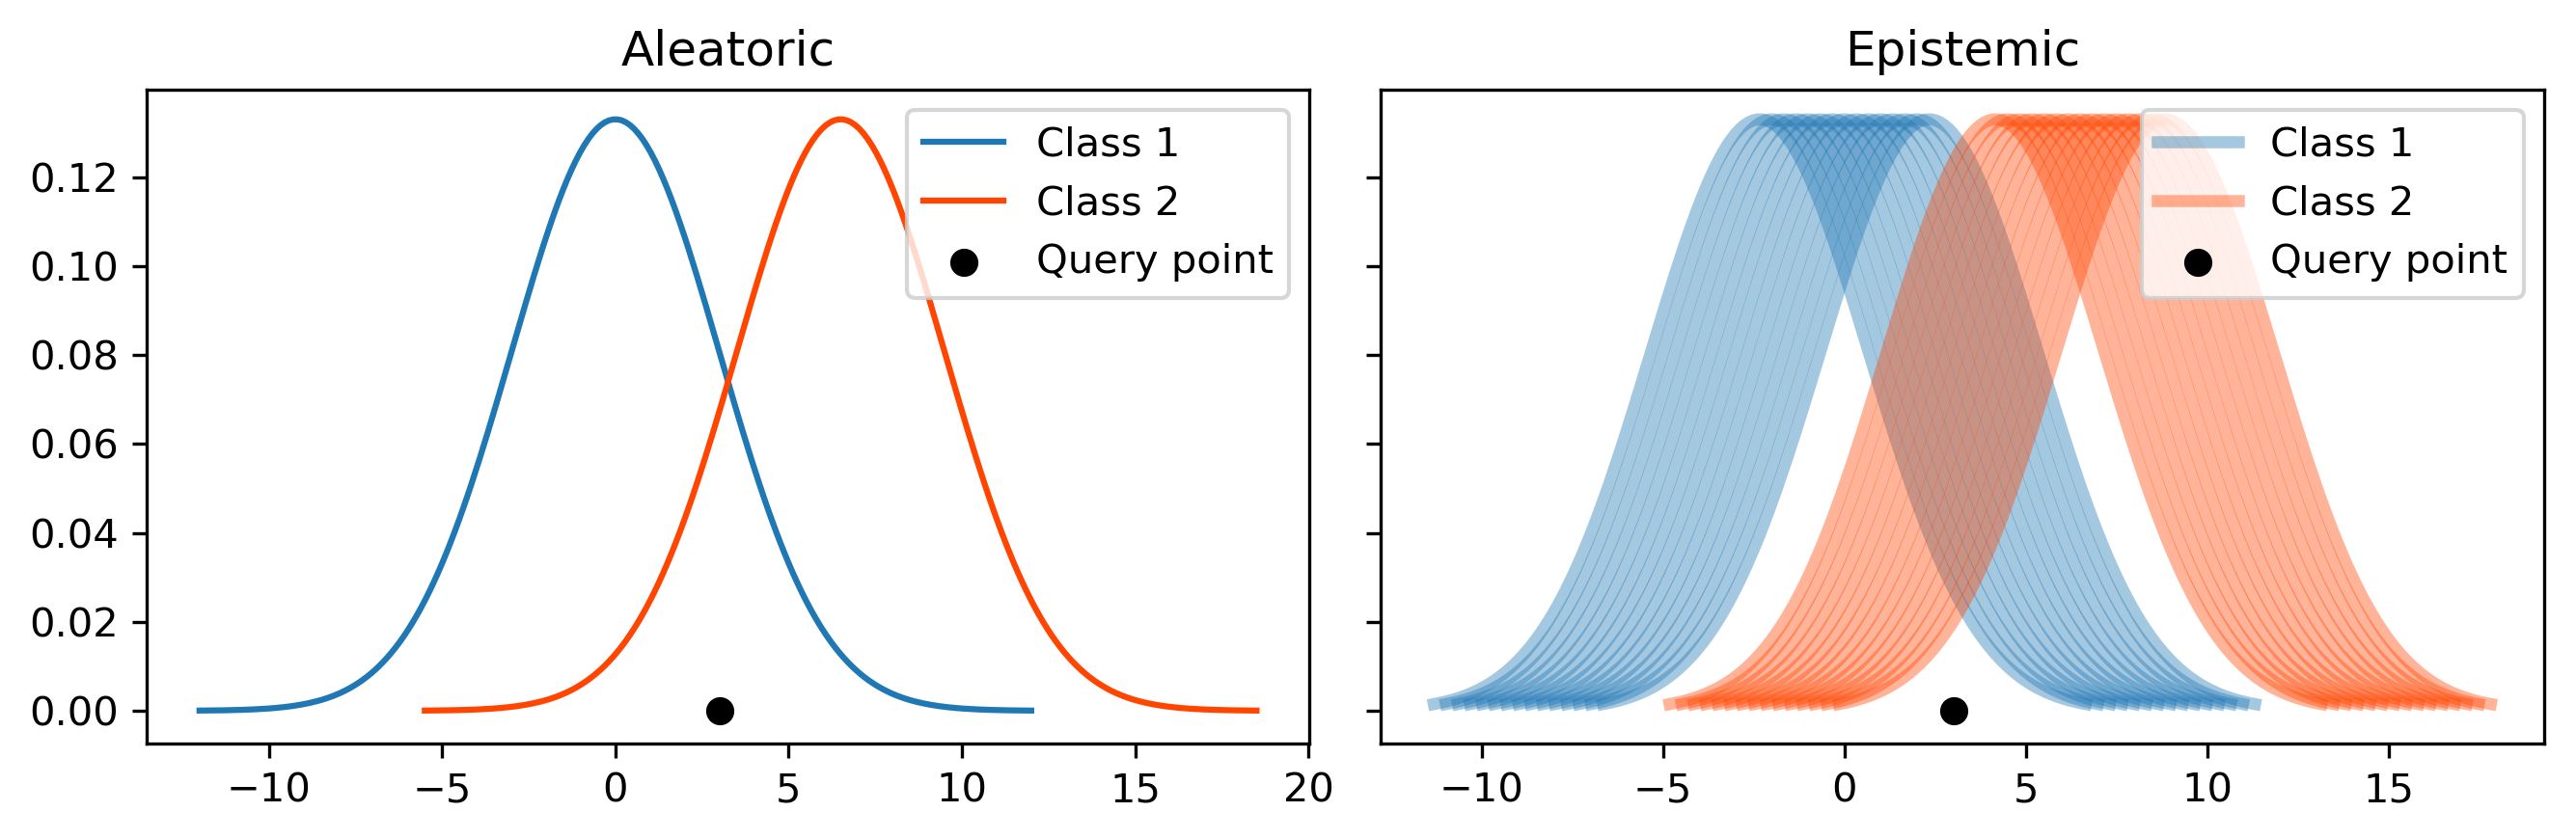
\includegraphics[width=1\textwidth]{Background/aleatoric_epistemic.png}
    \caption[Aleatoric vs. epistemic uncertainty]{A visual depiction of aleatoric and epistemic uncertainty. In the right plot, the query point has no epistemic uncertainty and high aleatoric uncertainty. In the left plot we have high epistemic uncertainty about the query point and its true aleatoric uncertainty is not known to us.}
    \label{fig:aleatoric_vs_epistemic}
\end{figure}

In this section, we will explore the sources of uncertainty in machine learning, following \citet{der2009aleatory} we break down uncertainty into

\begin{itemize}
    \item \textbf{Aleatoric uncertainty} or the "known-unknown" is uncertainty stemming from the stochasticity of the process we are modelling. Also referred to as the irreducible uncertainty, since we cannot reduce it by gathering more data. For example, data generated by balanced coin flips has high aleatoric uncertainty. We cannot be, certain of the outcome of the next flip, no matter how much data we collect about the coin. 

    \item \textbf{Epistemic uncertainty} is model uncertainty or the uncertainty which can be reduced by getting more knowledge. It denotes situations where we are uncertain as to what model generated the data.
    Note that unlike aleatoric uncertainty, this is primarily about our knowledge, rather than a property of the phenomenon we are modeling. For instance a heavily biased coin is initially high in epistemic uncertainty, but as we see more flips, we become more certain about the outcome of the next flip.
\end{itemize}

\Cref{fig:aleatoric_vs_epistemic} shows a depiction of both uncertainties in the context of classifying points sampled from two Gaussians. In the left plot, we see the true model which generated the data, yet we are uncertain about which class the query point came from. This is a depiction of high aleatoric uncertainty. 
In the right plot, we do not know the true model, we only have some prior guess over the Gaussians which generated the data, this is a situation with high epistemic uncertainty. Note that in this case, we do not know what the aleatoric uncertainty for the query point is. Depending on what the true model is, the aleatoric uncertainty may be high or low. 

We will explore each uncertainty in more detail, discuss its relevance to us, and see where it appears in the posterior predictive distribution. 


\subsection{Aleatoric Uncertainty}
\label{subsec:aleatoric}
Aleatoric uncertainty is the result of \pdf{y|x} being stochastic. For instance, in a classification problem with regions where classes overlap, such regions would have high aleatoric uncertainty, since it is impossible to determine the class for points from this region with 100\% accuracy. In our example of virtual sensors, the relationship between the inputs and outputs may be deterministic, but aleatoric uncertainty can arise due to noise; if the inputs have noise in them, it may not be possible to determine the exact output. Since we only see the noisy data, the process becomes stochastic from our perspective.
A distinguishing property of aleatoric uncertainty is that it is simply a property of the data, or the process which generated it \pdf{y|x}. It follows that unless we know a priori how it behaves, we must \emph{learn} it from the data. 

Thus to handle aleatoric uncertainty, we need models which can output probabilities rather than definite answers. For classification problems, the standard approach is to output a categorical distribution over the classes. For regression, a common approach is to output the mean and variance of a Gaussian distribution~\citep{kendall2017uncertainties, goodfellow2016deep}. 

Recall the posterior predictive 
$$
    \pdf{y|x; \mathcal{D}}=  \int \pdf{\theta | \mathcal{D}}\, \pdf{y|\theta, x} \, d\theta
$$

The aleatoric uncertainty comes from the individual models $\pdf{y|\theta, x}$. If the true model \pdf{y|x} is known, then we can perfectly predict the aleatoric uncertainty. However, the less we know about \pdf{x|y}, the less we are able to predict the aleatoric uncertainty. Note that this is different from \textbf{knowing} that we have high aleatoric uncertainty. 

Epistemic uncertainty represents our lack of knowledge about the true model \pdf{x|y}, when our epistemic uncertainty is high, we cannot make good predictions of the aleatoric uncertainty. In the next section we will discuss epistemic uncertainty, and where it fits in the Bayesian framework. 

\begin{figure}
    \centering
    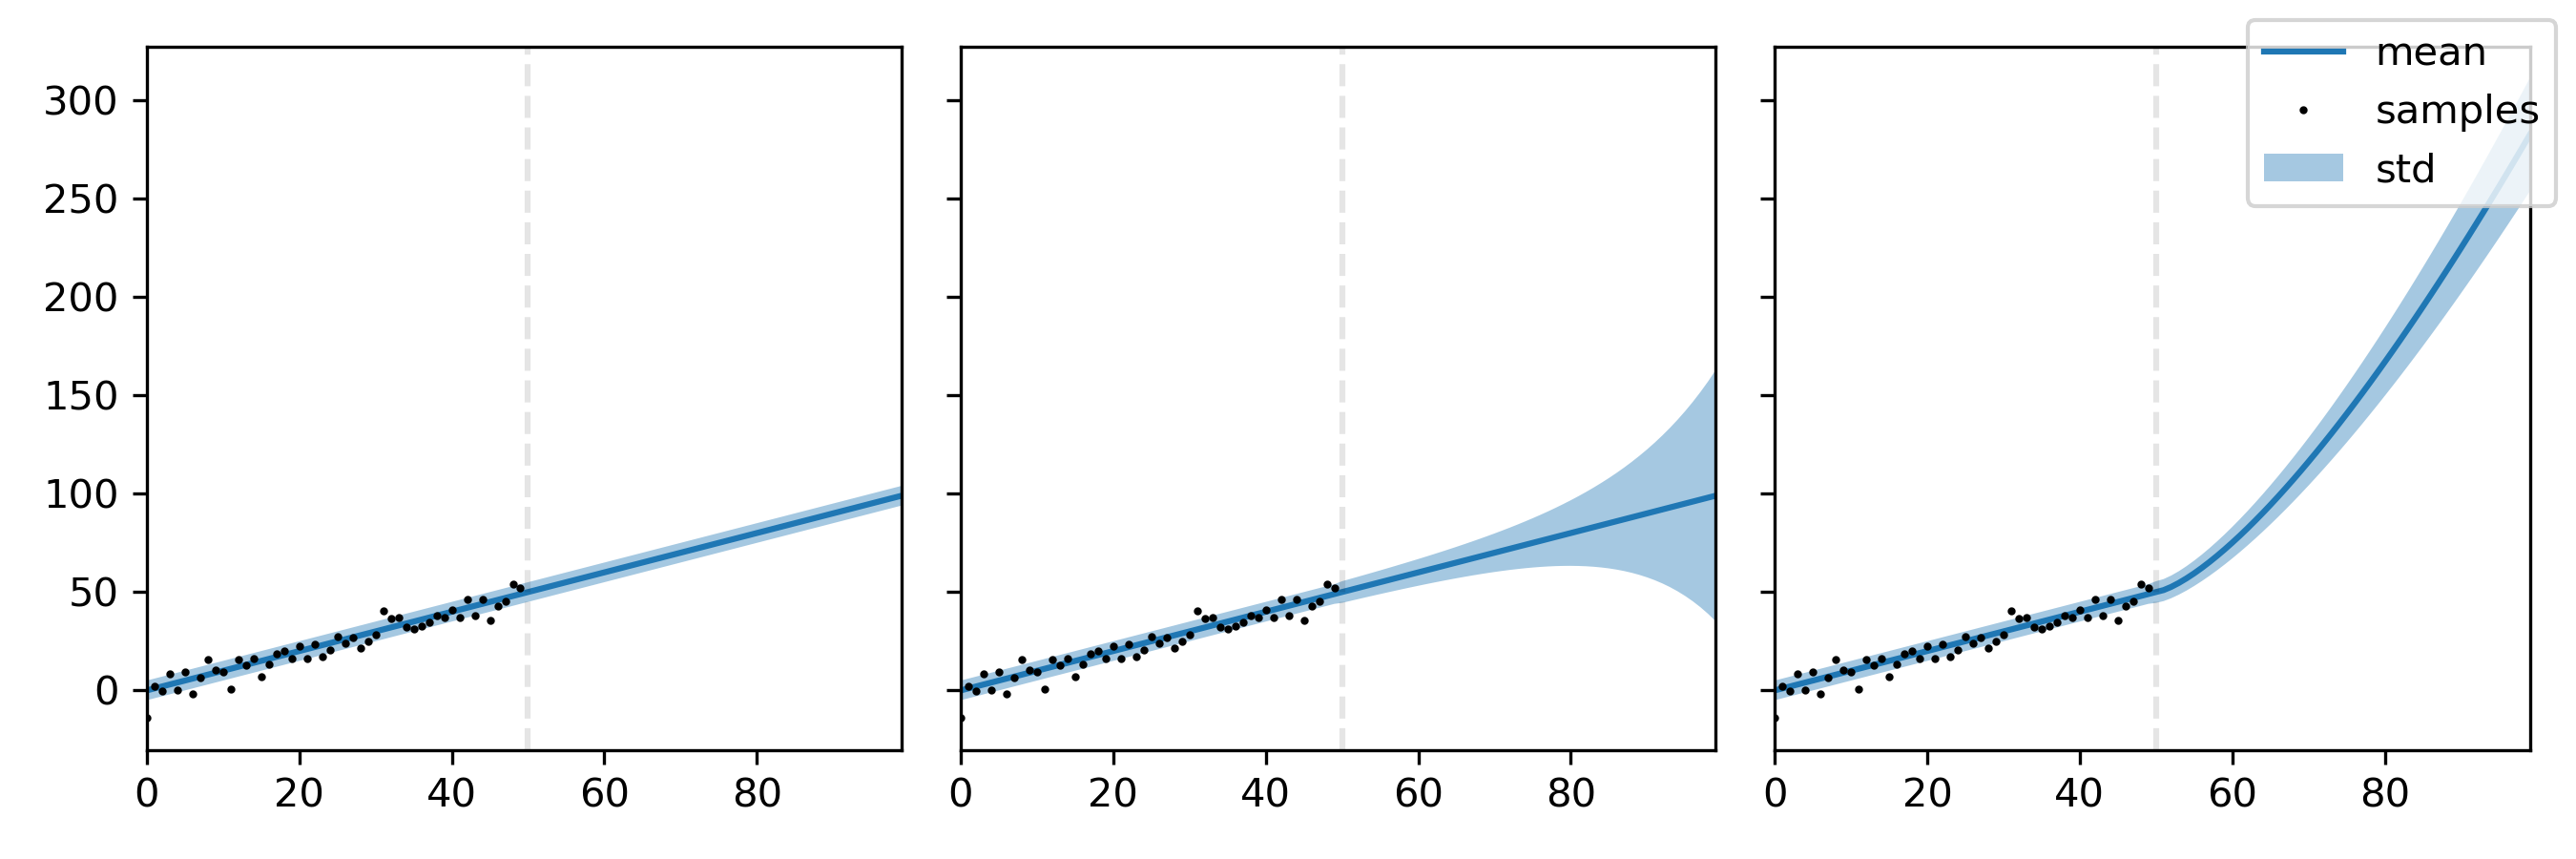
\includegraphics[width=1\textwidth]{Background/uncertainty_beliefs.png}
    \caption{Different beliefs equally consistent with the sampled data}
    \label{fig:uncertainty_toy}
\end{figure}

\subsection{Epistemic uncertainty}
\label{sec:epistemic}
Going back to the Bayesian framework, so far, we collected data about a phenomenon, used this data to update our prior belief into the posterior belief \cref{eq:bayes_rule}, then use the posterior to form our predictive distribution for new inputs \cref{eq:bayesian_predictive}.
Recall the posterior predictive
$$
    \pdf{y|x; \mathcal{D}}=  \int \pdf{\theta | \mathcal{D}}\, \pdf{y|\theta, x} \, d\theta
$$


The epistemic uncertainty comes from compounding two factors, the uncertainty in $\pdf{\theta | \mathcal{D}}$, and the \emph{disagreement} between the parameters with high posterior probability  $\pdf{\theta | \mathcal{D}}$. To unpack this, the uncertainty in $\pdf{\theta | \mathcal{D}}$ is simply how spread out the posterior is over different parameter settings. For instance, if the posterior is Gaussian, then the higher the variance of that Gaussian the higher the uncertainty is. However, the uncertainty over parameters does not directly translate into uncertainty in the posterior predictive distribution. This also depends on how much the predictions from those different parameters diverge. Being uncertain over a wide range of parameters which all give the same prediction, will result in no epistemic uncertainty in the predictive distribution. On the other hand, having a posterior concentrated over a few parameter settings which have large differences in their predictions can result in high epistemic uncertainty. In an ideal setting, the posterior predictive distribution captures all our epistemic uncertainty; \cref{eq:bayesian_predictive} gives the \emph{correct} predictive distribution.


\chmp{

Not sure talking about different distributions is all that clear. How about talking about the domain of the inputs and how your training data 
is sample of all possible inputs. And then you can introduce two distributions, one training and one at test time, say dry and snow, and argue
how it can be that they only have limited overlap. 

Then you can also avoid to same extent of having to introduce the "unversial" distribution and names for the distributions.

}

The Bayesian framework, alongside most other practical ML approaches~\citep[chapter~5]{goodfellow2016deep}, assume the training data is independently and identically distributed(i.i.d) from the target distribution, the target distribution being the one we intend to perform inference on. Problems arise when this assumption is broken.
Let the target distribution be $\pdf{x,y} = \pdf[target]{x} \pdf{y|x}$.
We consider a scenario where the training data is drawn i.i.d from a training distribution which is different form the target distribution, $\pdf{x,y} = \pdf[train]{x} \pdf{y|x}$. Thus the problem is that the distribution over the inputs is different from training to inference. 
Intuitively the image we have is that \pdf[target]{x} is a \emph{wider} distribution capturing all possible inputs, and \pdf[train]{x} concentrates its probability on a sub-region of \pdf[target]{x}. We refer to inputs which occur frequently in \pdf[target]{x} but not in \pdf[target]{x} as Out-Of-Distribution~(OOD).

The problem is that the model could be asked at inference time to make predictions over input regions where it has seen no data. \Cref{fig:uncertainty_toy} shows three possible posterior predictive distribution, all identical in the region from zero to fifty. We also have some training samples in that region. All three distributions are equally consistent with the data, so which one of those should we get if we ran a Bayesian learning algorithm on the data?

It depends on the priors and other underlying assumptions. If we choose the \emph{right} prior for our problem we may end up with a distribution that closely matches the true distribution we are modelling. However, if we do not know the right prior, we cannot be confident that we got a reasonable answer. Note that we are not only risking getting incorrect mean predictions, but also incorrect uncertainty estimates. Therein lies the problem with the Bayesian approach when the i.i.d assumption is broken. There is a component of uncertainty which is not accounted for. Note that this is not the case when data is i.i.d, where with enough data, a poor choice of prior can be overcome. 


% \chmp{
    
%     I got confused by looking at the wrong figure first. However, I also believe that you can make your argument strong by
%     switching the discussion around. First start with a dataset and the two different sampling processes for the training data.
%     And then discuss the potential beliefs about the unseen points that are compatible with the observed data in case of the right 
%     example. (I.e., there is only one dataset, but different beliefs about unseen data).
    
%     Why are there different datasets? And why does the conditional distribution differ? If you assume $P(y|x)$ is the 
%     data generating process, there is no need to assume the generative process changes between intervals, but only that 
%     we have limited knowledge.
    
%     I would frame the whole discussion in the way of talking about a underlying data generating process, but different ways
%     to sample the training data. I.e., there is only one true curve, but in the right example we only see the linear part,
%     in the left example we see the samples from the whole domain.
    
%     I also have the impression that you are repeating yourself a couple of times. If you wanted to, you should be able to shorten
%     the section.
% }

% \Cref{fig:uncertainty_toy} shows samples from three datasets. The universal input distribution \dist{u} is the same for all three. 
% We split the input domain into two intervals, then we define \pdf{y|x} to be the same for all three datasets in the first interval, but different in the second. 
% Specifically, the black points, in the interval between zero and fifty, are sampled from the same \pdf{y|x} for all three datasets. The function is simply a line with slope one and small Gaussian noise added. The red points, in the interval between fifty and a hundred, have a different dynamics for each dataset. 

% In the first dataset(right) the red points continue along the same line. In the second dataset also they also continue linearly but the scale of the Gaussian noise increases exponentially as we move along the x-axis, i.e the mean of \pdf{y|x} continues to be the same but the variance changes. For the last dataset, the red points grow polynomially i.e the mean of \pdf{y|x} diverges from the first two datasets. Note that this data represents the ground truth, so in dataset 2 for example the aleatoric uncertainty increases rapidly as we move up the x-axis.

% If we constrain our training samples to be drawn from a training \pdf[t]{x} which only covers the black region, then it is unclear from the data what are the \emph{correct} outputs for the red region. Any solution which is well suited for one of the datasets is unsuitable or at least sub-optimal for the other two, yet the training data is identical. Note that this holds even if we follow the full Bayesian approach. 

To illustrate the difference, we take one i.i.d sampling and one biased sampling from a ground truth function which looks like the leftmost plot in \cref{fig:uncertainty_toy} and fit a Bayesian model to both. We used the bayesian ridge regression from scikit learn\citep{scikit-learn}, with the default hyper-parameters in both cases. Everything is the same, with the exception that the distribution over training inputs.

\Cref{fig:bayesian_ridge} shows the results. The shaded region represents the epistemic uncertainty 
\chmp{Does it though? I understood your argument above that there is a very specific part of a Bayesian model that is responsible for the epistemic uncertainty, I assume you plotted the combined uncertainty, didn't you?}
\ahmed{There is no aleatoric uncertainty in this model, each individual model is deterministic}
, it is two standard deviations wide. We can see that in the case of biased samples the model severely underestimates the uncertainty, with the points above ninety lying roughly eight standard deviations away from the mean. Note that we are not focused about the magnitude of the error, but on the high degree of certainty with which it is made i.e. if the error was the same, but the standard deviation was eight times larger, we could say that the model did well in estimating the uncertainty. 

\begin{figure}
    \centering
    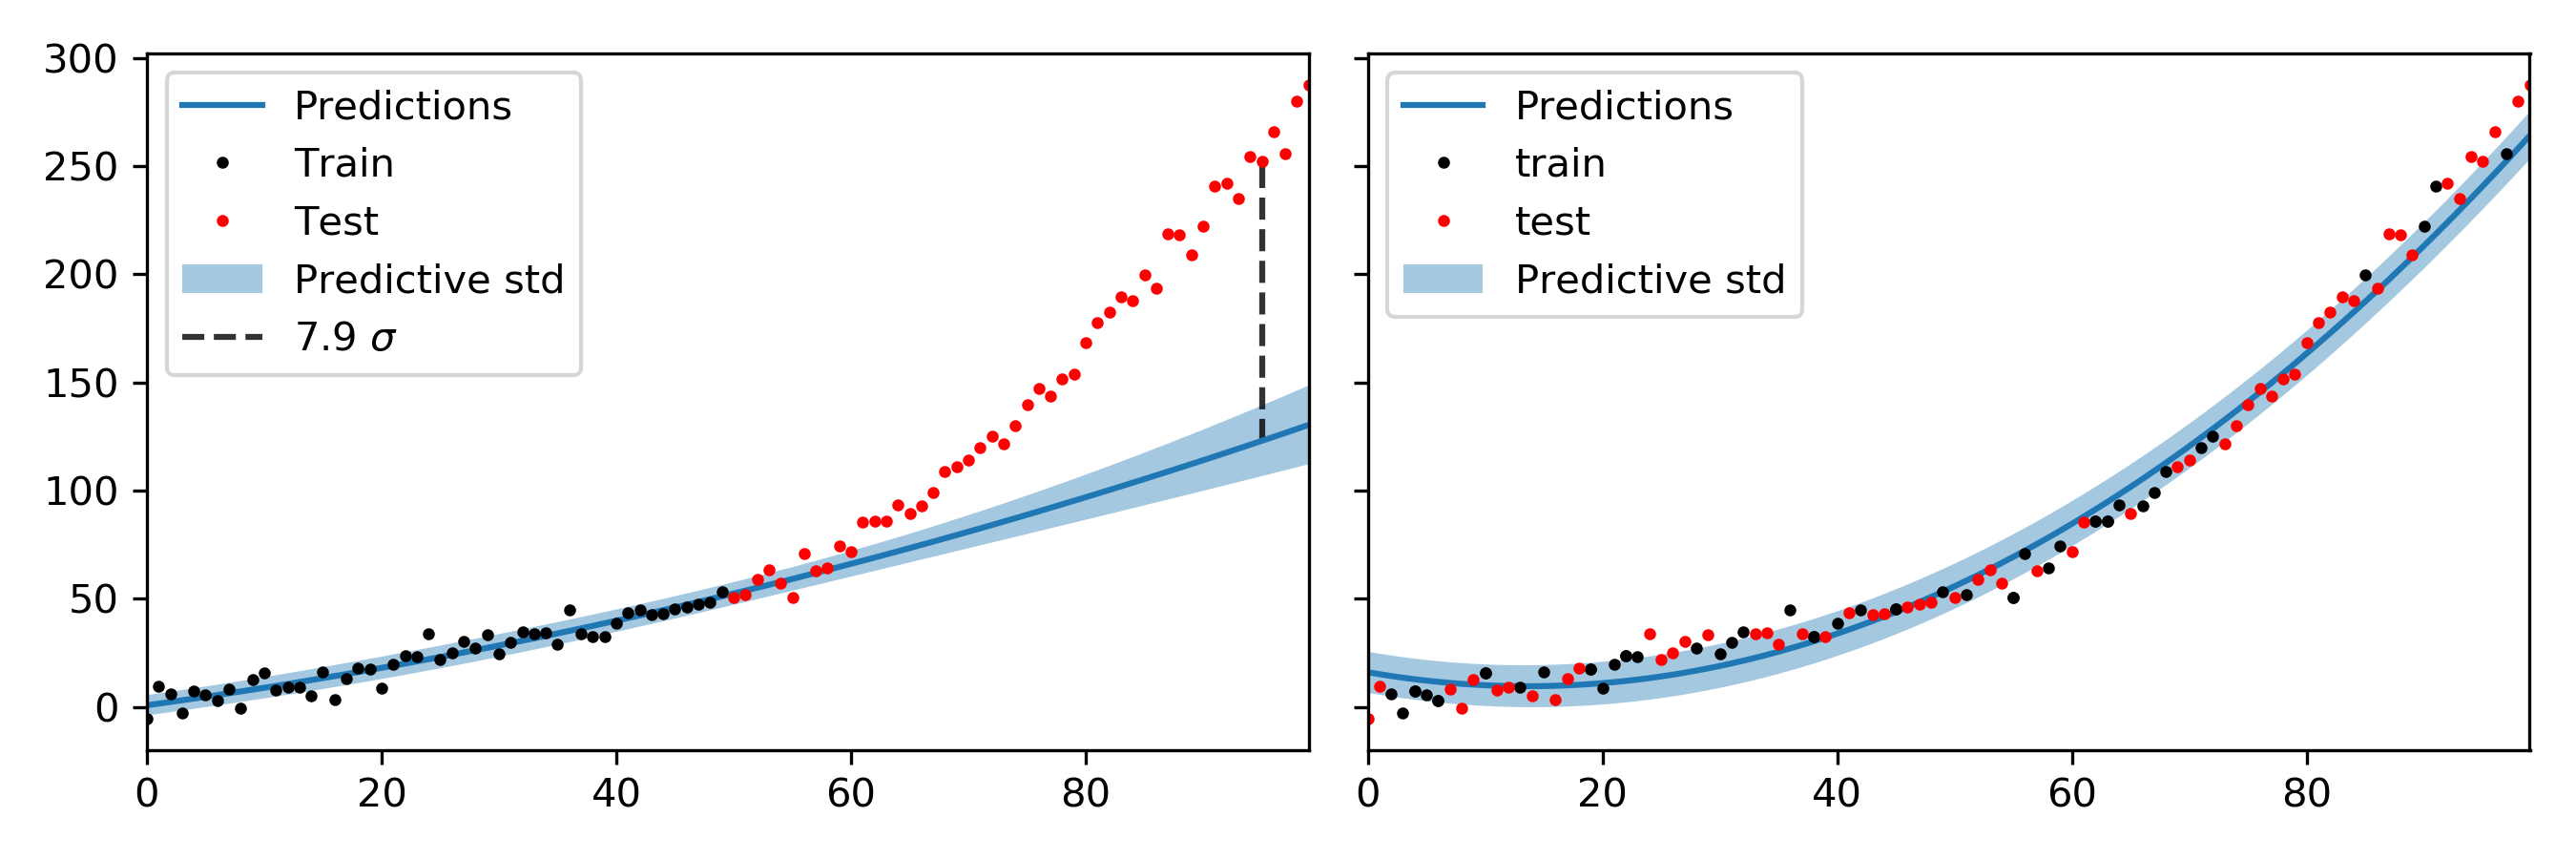
\includegraphics[width=1\textwidth]{Background/BayesianRidge2.png}
    \caption{Quadratic Bayesian regression fitted on different samples from the same dataset}
    \label{fig:bayesian_ridge}
\end{figure}

The models shown in \cref{fig:bayesian_ridge} the models were both trained with fifty samples, which may seem unfair to the model with biased sampling. 
To further highlight the importance of the i.i.d assumption, \cref{fig:bayesian_ridge_low}, shows the two runs of the same model, each trained with only ten i.i.d samples. With only one fifth of the number of samples, we still get decent results, provided they are i.i.d. On the other hand, when the training data does not cover a certain region of input space, we cannot trust the epistemic uncertainty as estimated by \cref{eq:bayesian_predictive}.

\begin{figure}
    \centering
    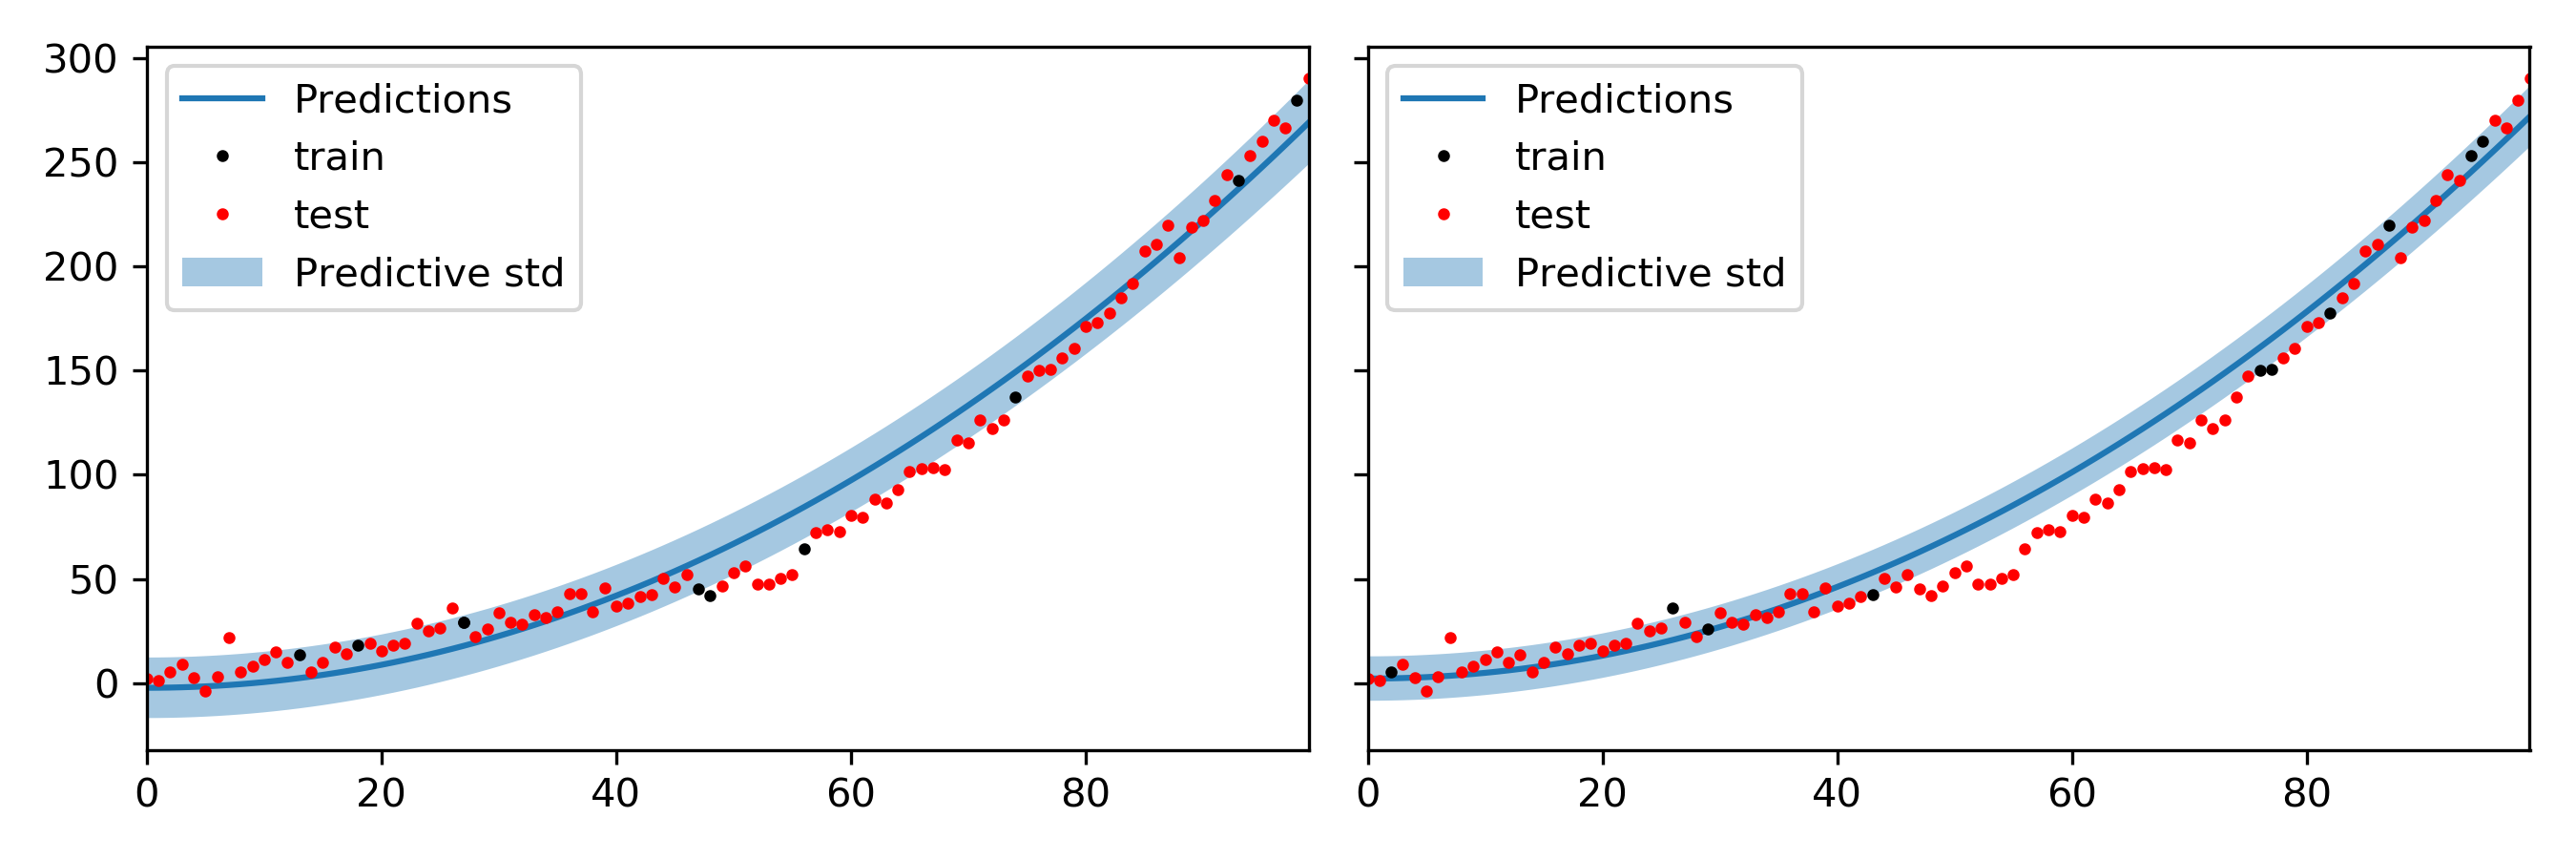
\includegraphics[width=1\textwidth]{Background/BayesianRidgeLow.png}
    \caption{Quadratic Bayesian regression fitted with only 10 i.i.d samples}
    \label{fig:bayesian_ridge_low}
\end{figure}


In our running example of estimating vehicle velocity from sensor measurements. 
\chmp{If you use the running example, you should have introduced the problem, but maybe you do not need to be so specific and just talk about the general behavior of a vehicle}.
Suppose we train a model using data collected on dry roads. the car driving on icy roads is an example of being OOD.
The question again is how valid is our estimate of epistemic uncertainty for OOD inputs. Let us take the case where our hypothesis space contains a model perfect on dry roads, another perfect on icy roads, and all other models have decent performance over both. Assume a uniform prior. Training on dry roads data alone, we eventually end up placing all the posterior mass on the dry roads models.
This drives our epistemic uncertainty, as estimated in \cref{eq:bayesian_predictive}, down to zero everywhere. This means we will be making confident predictions on icy roads, although our predictions for icy road are potentially inaccurate. 

The takeaway is that our uncertainty estimate is not complete for OOD data. The model will be confidently wrong on icy roads. How much we can trust this estimate in practice depends on the hypothesis space, priors, and the behavior of \pdf{y|x}. In the next section, we will formalize the learning setting we discussed here, and discuss a principled approach to handling it.







\subsubsection{Formalizing the problem}
\label{sec:formalizing}

In the previous section, we described a situation where the training and target distribution do not match up, we have seen that the Bayesian framework may produce overconfident results in such situations. In this section we will formalize this setting and give it a principled treatment. Our focus will be on obtaining sound uncertainty estimates. This section is our own novel work, it is not a standard approach to the best of our knowledge. 

As before, we have a supervised training setting, where we get some training samples from a joint \pdf[train]{x,y}, where $x$ is the input, and $y$ is the target, and we wish to model the conditional \pdf{y|x}. We decompose the joint $\pdf[train]{x,y} = \pdf[train]{x} \pdf{y|x}$ using the product rule~\citep[chapter~2]{mackay2003information}, during inference we get samples from another input distribution $x\sim\pdf[target]{x}$, and we wish to make a prediction for \pdf{y|x}. 

Let us define this target distribution as a mixture of the training distribution and some other distribution such that

\begin{equation}
    \pdf[target]{x} = \pdf{z=0} \pdf{x|z=0} + \pdf{z=1} \pdf[]{x|z=1}
\end{equation}{}

where $z$ is a binary random variable denoting which distribution the input is sampled from, so that \pdf[train]{x} = \pdf[]{x|z=1}, and \pdf[other]{x} = \pdf[]{x|z=0}. 
% This means that at inference time, a bent coin~\citep[chapter~2]{mackay2003information} is flipped and the input is sampled from the corresponding distribution.
Note that if we set \pdf{z=0} to zero, we get back the typical i.i.d framework, so this is an extension.

Now we will suppose we got the training data $\mathcal{D}$, preformed the learning and ended up with some posterior distribution, we will use the parameters $\Theta$ as a shorthand for the model defining the posterior predictive distribution
$$
    \pdf{y|x; \Theta}=  \int \pdf{\theta | \mathcal{D}}\, \pdf{y|\theta, x} \, d\theta
$$
$\Theta$ basically contains all the knowledge we gained from the training data. For samples from \pdf[]{x|z=1}, $\Theta$ is the parameter vector we want to use for inference. However, we have not used any samples from the other distribution \pdf[]{x|z=1} when learning $\Theta$, and this is the reason using $\Theta$ for those inputs may lead to incorrect results, like the overconfident mistakes we saw in \cref{fig:bayesian_ridge}. 

As we see no data from the other distribution \pdf{x|z=0}, we will define a model with parameters $\Psi$. This model should be our best knowledge about \pdf{y|x} over the distribution \pdf{x|z=0}. 
Now we have two models $\Theta$ and $\Psi$, to make predictions we form a posterior predictive distribution
$$
    \pdf{y|x} = \pdf{\Theta|x} \pdf{y| x; \Theta} + \pdf{\Psi|x} \pdf{y | x; \Psi}
$$

We will make the simplifying assumption that $\Theta$ is the right model for points coming from the training distribution, and $\Psi$ is the right model for points coming from the other distribution. The means that \pdf{\Theta|z=1} and \pdf{\Psi|z=0} are set to one; if we know which distribution the point came from, we know which model to use for prediction. This means that we can write
\begin{equation}
    \label{eq:simplifying}
    \pdf{\Theta|x} = \pdf{z=1|x} ;\,\,\, \pdf{\Psi|x} = \pdf{z=0|x}
\end{equation}{}

With this we can rewrite the posterior predictive as
\begin{equation}
    \label{eq:final_posterior}
    \pdf{y|x} = \pdf{z=1|x} \pdf{y| x; \Theta} + \pdf{z=0|x} \pdf{y | x; \Psi}
\end{equation}{}

To find \pdf{z=1|x}, and we can use Bayes rule
$$ 
    \pdf{z|x} = \frac{\pdf{x|z} \, \pdf{z}}{\pdf{x}}
$$

This gives us a sound framework for preforming inference in the scenario we described, under the assumption made in \cref{eq:simplifying}. The problem is that there are quantities in there which we cannot estimate from the training data, namely \pdf{z}, \pdf{x|z=1}, and the parameters $\Psi$. \pdf{z} can be treated as a hyperparameter and \pdf{x|z=1} can be defined as a generic distribution suitable for the application at hand.

The parameters $\Psi$ defines a predictive model for regions where we have not seen data. In the previous section, we claimed that predictions from a Bayesian ensemble cannot be trusted in OOD regions, this should clarify why. The ensemble would be implicitly assuming some $\Psi$, based on the combination of priors and underlying assumption we put in. In some cases this may yield good results, but it cannot be trusted in general. 

The parameters $\Psi$ can simply be chosen to increase uncertainty in some sense. For instance, in a classification problem we can let $\Psi$ define a model which outputs a uniform distribution over the classes. This will simply act as a smoother for the classifier, and the farther we move from the training distribution the more uniform model predictions will become. 

For regression, suppose our model outputs $\mu_\Psi$ and $\sigma_\Psi$ as parameters of a Gaussian. We may define the model to output a unit Gaussian s.t. \pdf{y|, x, \Psi} = $\mathcal{N}(y; 0, 1)$. We could also use richer prior knowledge. Let $\pdf{y|x, \Theta} = \mathcal{N}(y; \mu_y, \sigma_y)$. We can then define $\pdf{y|x, \Psi} = \mathcal{N}(y; \mu_y, \sigma_\Psi)$, with $\sigma_\Psi$ being a hyper-parameter. This model assumes that our best guess for an OOD input is still the mean prediction from the trained model, however with more uncertainty. 
% This is in fact the model , noise contrastive priors~\citep{Hafner2018NoiseCP}.

This framework requires substantial prior knowledge, which depending on the context can be a challenge or an opportunity. Intuitively, this prior knowledge is required to fill the gaps we are left with due to breaking the i.i.d assumption. 

In this work we will not focus on designing the priors, but rather on the one central quantity of this framework which can be learned from data: \pdf[train]{x}. This probability is central to computing the posterior predictive distribution we proposed in \cref{eq:final_posterior}. Intuitively, the higher the probability of an input under the training distribution, the more weight we give to $\Theta$ the model learned under the training distribution. The probability of the input alone is not sufficient to make a full prediction.

However, there are works in current machine learning which aim to estimate \pdf[train]{x}, and simply return this as a signal for whether the model's prediction can be trusted~\citep{vasilev2018q, pidhorskyi2018generative}. This will be our strategy. Our experimental results in \cref{ch:experiments}, support the claim that the model's errors do correlate inversely with the probability of the input, and that excluding low probability inputs is a practical strategy for pruning out unreliable predictions. 

In the next chapter, we will present our compression RNNs, which can effectively learn to estimate the training distribution density for temporal data and give a strong predictive performance.  

  

% \subsection{Closing thoughts}

% \chmp{Why discussion here? You have discussed quite a lot in the other parts already.}
% \ahmed{is closing thoughts better? Summary? }

% In the general case, we only gain knowledge about our target function \pdf{y|x} in regions of $x$ covered by the training distribution. 

% In the general case, we can only trust model predictions in input regions covered by the training distribution. Outside this distribution, aleatoric uncertainty is unknown to us, as it is a property of \pdf{y|x} which we try to learn from data 
% \chmp{If you go Bayes, you only learn the parameters (or distributions over them). I had the impression, you were comitting yourself to a Bayes approach.}
% \ahmed{Aleatoric uncertainty is a prediction from the individual models, it has nothing to do with going Bayes or not. In our case it is represented by the variance of the Gaussian which our network outputs. (cf. \cite{kendall2017uncertainties}) they do the dropout + aleatoric uncertainty}
% , and as such cannot know its behavior in regions far away from the data we see; we do not know the aleatoric uncertainty in those regions. 

% Since the problem is our lack of knowledge about \pdf{y|x} in those regions, it is the epistemic uncertainty that should capture this.
% But epistemic uncertainty, as estimated in the standard bayesian framework, can mislead us, since the posterior may become too concentrated on a narrow set of models which perform well on \dist{t}, although they could be performing arbitrarily worse on the rest of \dist{u}.  

% We've argued that outside the training distribution, the standard uncertainty framework in ML fails to soundly account for the uncertainty. 
% Our estimates of the two components of uncertainty fail to fully capture the uncertainty, and can be arbitrarily wrong. In fact, as we move far from the training distribution, the true magnitude of our uncertainty cannot be predicted from the training data. As \cref{fig:uncertainty_toy,fig:bayesian_ridge}
% demonstrate, the behavior away from the training distribution could be anything, and training samples cannot tell us anything about it. As such, any model estimating the predictive uncertainty(e.g. variance around the mean or confidence intervals) outside the support of the training distribution is relying more on priors, often implicit ones, rather than on the data. 

% \chmp{Since this idea is known, I would add a citation. + I would consider discussing it already earlier. }

% In the absence of strong priors, one solution is to only make confident predictions in regions well covered by the training distribution. We would argue that ideally the model should have a separate output denoting whether or not an input is in the region where the model is valid. This amounts to estimating whether or not an input has likely come from the training distribution. Such models do not actually give predictive uncertainty estimates, like a variance around the prediction, but only tell us how likely would the model be valid for a particular input. Moreover, such estimates can be used to form predictive uncertainties, but require some prior knowledge to be explicitly defined. 

% % Learning to estimate uncertainty from data makes the line between the our components of uncertainty fuzzy. Most notable, while aleatoric uncertainty should be independent of the our knowledge and priors, in practice when we learn to predict it from data

% In the following section, we will present our approach for prediction and uncertainty estimation on time series data. We will also present a principled method to forming sound predictive uncertainties on OOD inputs when the appropriate priors are available. Then we will present the results of our models on vehicle dynamics problems. 

\end{document}
